\documentclass[14pt, xcolor={usenames, dvipsnames}]{beamer}
%\documentclass[handout, 14pt, xcolor={usenames, dvipsnames}]{beamer}

\usepackage{etex}
\usepackage[english]{babel}
\usepackage[utf8]{inputenc}
\usepackage[T1]{fontenc}
\usepackage{mathptmx} % Times Roman clone
\usepackage{amsfonts}
\usepackage{amsmath}
\usepackage{amssymb}
\usepackage{graphicx}
\usepackage{hyperref}
\usepackage{booktabs}
\usepackage[round]{natbib}
\usepackage{tikz}
\usepackage[labelformat=empty]{caption}
\usepackage{colortbl}
\usepackage{ulem}
\usepackage{multicol}
\usepackage[overlay]{textpos}
\usepackage{multirow}
\usepackage{ifthen}
\usepackage{relsize}
\usepackage{ragged2e}
\usepackage{rotating}

\usetheme{Boadilla}
\setbeamercovered{transparent}
\setbeamertemplate{frametitle continuation}{}
\setbeamertemplate{sections/subsections in toc}[square]
\setbeamertemplate{blocks}[rounded][shadow=false]
\setbeamertemplate{footline}{\vskip2pt}
\setbeamertemplate{enumerate items}[square]
\setbeamertemplate{itemize item}{\footnotesize$\blacksquare$}
\setbeamertemplate{itemize subitem}{\scriptsize$\blacktriangleright$}
\beamertemplatenavigationsymbolsempty

\usetikzlibrary{positioning, topaths, shapes, arrows}
\newcount\mycount           % TopicRank slides
\newcommand{\pagerank}[1]{  % TopicRank slides
  \ifthenelse{\equal{#1}{1}}{
      2.673
  }{
    \ifthenelse{\equal{#1}{2}}{
        2.237
    }{
      \ifthenelse{\equal{#1}{3}}{
          2.285
      }{
        \ifthenelse{\equal{#1}{4}}{
          1.451
        }{
          \ifthenelse{\equal{#1}{5}}{
            0.612
          }{
            \ifthenelse{\equal{#1}{6}}{
              1.017
            }{
              \ifthenelse{\equal{#1}{7}}{
                0.405
              }{
                \ifthenelse{\equal{#1}{8}}{
                  0.717
                }{
                  \ifthenelse{\equal{#1}{10}}{
                    0.749
                  }{
                    \ifthenelse{\equal{#1}{11}}{
                      0.600
                    }{
                      \ifthenelse{\equal{#1}{12}}{
                        0.750
                      }{
                        \ifthenelse{\equal{#1}{13}}{
                          0.575
                        }{
                          \ifthenelse{\equal{#1}{14}}{
                            0.669
                          }{
                            \ifthenelse{\equal{#1}{15}}{
                              0.615
                            }{
                              \ifthenelse{\equal{#1}{16}}{
                                1.112
                              }{
                                \ifthenelse{\equal{#1}{17}}{
                                  0.455
                                }{
                                  \ifthenelse{\equal{#1}{18}}{
                                    0.697
                                  }{
                                    0.600
                                  }
                                }
                              }
                            }
                          }
                        }
                      }
                    }
                  }
                }
              }
            }
          }
        }
      }
    }
  }
}

\renewcommand\cite[2][]{\citep[#1]{#2}}
\let\oldtextsc\textsc\renewcommand\textsc[1]{\rmfamily\oldtextsc{#1}}

\title{TopicRank}
\subtitle{Graph-Based Topic Ranking for Keyphrase Extraction}
\titlegraphic{
  \begin{center}
    
\includegraphics[height=1.75em]{logos/ijcnlp.eps}\hfill
    
\includegraphics[height=1.75em]{logos/univ_nantes.eps}\hfill
    
\includegraphics[height=1.75em]{logos/lina.eps}\hfill
    
\includegraphics[height=1.75em]{logos/termith.eps}\hfill
  \end{center}
}
\author{\textbf{Adrien Bougouin} \and Florian Boudin \and Béatrice Daille}
\institute{\normalsize{Université de Nantes, LINA, France}}
\date{16 October 2013}

\begin{document}
  \renewcommand*{\theenumii}{\alph{enumii}}
  \renewcommand*{\theenumiii}{\roman{enumiii}}
  \addtobeamertemplate{block begin}{\setlength\abovedisplayskip{0pt}}

  \begin{frame}
    \titlepage
  \end{frame}
  \setbeamertemplate{footline}{\hfill\textbf{\textcolor{blue}{\insertframenumber{\ \ }}}\vskip2pt}
  \setcounter{framenumber}{0}

  \section{Introduction}
\label{sec:introduction}
  % * définition de terme-clé, applications et enjeux
  Un terme-clé est un mot ou une expression polylexicale qui représente un
  concept important d'un document auquel il est associé. En pratique, plusieurs
  termes-clés représentant des concepts différents sont associés à un même
  document. Ils forment alors un ensemble de termes-clés à partir duquel il est
  possible de déduire le contenu principal du document. Du fait de leur capacité
  à synthétiser le contenu d'un document, les termes-clés sont utilisés dans
  diverses applications en Recherche d'Information (RI)~: résumé
  automatique~\cite{avanzo2005keyphrase}, classification de
  documents~\cite{han2007webdocumentclustering}, indexation
  automatique~\cite{medelyan2008smalltrainingset}, etc. Avec l'essor du
  numérique, de plus en plus de documents (articles scientifiques, articles
  journalistiques, etc.) sont accessibles depuis des médiums d'informations tels
  que Internet. Afin de permettre à un utilisateur de rapidement trouver des
  documents, ainsi que d'avoir un bref aperçu de leur contenu, les tâches
  sus-mentionnées sont nécessaires.
  Cependant, la majorité des documents ne sont pas associés avec des termes-clés
  et, compte tenu du nombre important de documents numériques, l'ajout manuel de
  ces derniers n'est pas envisageable. Pour pallier ce problème, de plus en plus
  de chercheurs s'intéressent à l'extraction automatique de termes-clés et
  certaines campagnes d'évaluations, telles que DEFT~\cite{paroubek2012deft} et
  SemEval~\cite{kim2010semeval}, proposent des tâches d'extraction automatique
  de termes-clés.

  % * qu'est-ce que l'extraction automatique de termes-clés
  % * deux écoles : indexation libre et indexation contrôlée (assignation de
  %                 termes-clés)
  %   -> nous sommes de la première école
  % * deux catégories de méthodes : supervisées et non-supervisées
  %    -> en supervisé ils utilisent la structure des documents
  %    -> très peu de travaux en non-supervisé (filtrage des candidats)
  L'extraction automatique de termes-clés, ou indexation libre, est la tâche qui
  consiste à extraire les unités textuelles les plus importantes d'un document,
  en opposition à la tâche d'assignation automatique de termes-clés, ou
  indexation contrôlée, qui consiste à assigner des termes-clés à partir d'une
  terminologie donnée~\cite{paroubek2012deft}. Parmi les méthodes d'extraction
  automatique de termes-clés existantes, nous distinguons deux catégories~: les
  méthodes supervisées et les méthodes non-supervisées. Dans le cas supervisé,
  la tâche d'extraction de termes-clés est considérée comme une tâche de
  classification binaire~\cite{witten1999kea}, où il s'agit d'attribuer la
  classe \og{}\textit{terme-clé}\fg{} ou \og{}\textit{non terme-clé}\fg{} aux
  termes-clés candidats extraits du document. Une collection de documents
  annotés en termes-clés est alors nécessaire pour l'apprentissage d'un modèle
  de classification reposant sur divers traits, allant de la simple fréquence
  aux informations structurelles du document (titre, résumé, introduction,
  conclusion, etc.). Dans le cas non-supervisé, les méthodes attribuent un
  score d'importance à chaque candidat en fonction de divers indicateurs tels
  que la fréquence et la position de la première occurrence dans le document.
  Bien que les méthodes supervisées soient en général plus performantes, la
  faible quantité de documents annotés en termes-clés disponibles, ainsi que la
  forte dépendance des modèles de classification au type des documents à partir
  desquels ils sont appris, poussent les chercheurs à s'intéresser de plus en
  plus aux méthodes non-supervisées.

  % * ici, on cherche à identifier l'échelle de difficulté d'indexation des
  %   documents en Sciences Humaines et Sociales (SHS)
  % * on dispose de 4 collections de notices de 4 disciplines différentes de
  %   SHS + 1 collection de notices de chimie (science dure)
  Dans cette article, nous nous intéressons à l'extraction non-supervisée de
  termes-clés dans les articles scientifiques, et plus particulièrement à la
  performance des méthodes d'extraction de termes-clés dans des domaines de
  spécialité. Au moyen de cinq corpus disciplinaires, notre objectif est
  d'observer et d'analyser l'échelle de difficulté pour l'extraction
  automatique de termes-clés dans des articles scientifiques appartenant à cinq
  disciplines différentes~: Archéologie, Sciences de l'Information,
  Linguistique, Psychologie et Chimie.
  \TODO{Dire pourquoi nous nous intéressons aux méthodes non-supervisées}
  \TODO{Dire pourquoi nous nous intéressons aux articles scientifiques}

  % * annonce du plan
  L'article est structuré comme suit. Un bref état de l'art est donné dans la
  section~\ref{sec:etat_de_l_art}, les données utilisées sont présentées dans la
  section~\ref{sec:presentation_des_donnees} et les expériences menées, ainsi
  que les résultats obtenus, sont décrits dans la section~\ref{sec:experiences}.
  Enfin, une analyse des résultats est donnée dans la
  section~\ref{sec:discussion}, puis une conclusion générale et des perspectives
  de travaux futurs sont présentés en
  section~\ref{sec:conclusion_et_perspectives}.


  %\section{Related Work}
  \begin{frame}{Related Work}
    \framesubtitle{Unsupervised Methods}

    Mostly ranking technics using:
    \begin{itemize}
      \item{language models}
      \item<2->{clusters}
      \item<3->{or \textbf{graphs} of word
                co-occurrences}
      \begin{itemize}
        \item<4->{weighted with co-occurrence number or semantic measure}
        \item<5->{refined with similar documents}
        \item<6->{biased with topic probabilities}
      \end{itemize}
    \end{itemize}
    \vfill
    \alt<6>{
      \cite{liu2010topicalpagerank}
    }{
      \alt<5>{
        \cite{wan2008expandrank}
      }{
        \alt<4>{
          \cite{wan2008expandrank, tsatsaronis2010semanticrank}
        }{
          \alt<3>{
            \cite{mihalcea2004textrank}
          }{
            \alt<2>{
              \cite{liu2009keycluster}
            }{
              \cite{tomokiyo2003languagemodel}
            }
          }
        }
      }
    }
  \end{frame}

  \begin{frame}{Related Work}
    \framesubtitle{Graph-Based Approach: Example (TextRank) and Drawbacks}

    \begin{columns}
      \begin{column}{.6\textwidth}
        \centering
        \alt<3->{
          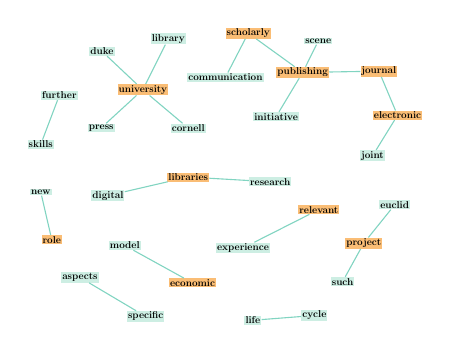
\begin{tikzpicture}[thin,
                              auto,
                              scale=.25,
                              align=center,
                              node distance=2cm,
                              every node/.style={font=\small, transform shape},
                              main node/.style={text centered,
                                                thick,
                                                fill=JungleGreen!20,
                                                inner sep=1.5pt,
                                                font=\Large\bfseries}]
            % connected component
            \node[main node, fill=BurntOrange!50] (university) {university};
            \node[main node] (duke) [above left=of university.north] {duke};
            \node[main node] (library) [above=of university.north east] {library};
            \node[main node] (press) [below left=of university.south] {press};
            \node[main node] (cornell) [below right=of university.south] {cornell};

            \path[JungleGreen!50] (university) edge (library);
            \path[JungleGreen!50] (university) edge (duke);
            \path[JungleGreen!50] (university) edge (press);
            \path[JungleGreen!50] (university) edge (cornell);

            % connected component
            \node[main node] (further) [left=of university.south west] {further};
            \node[main node] (skills) [below=of further.south west] {skills};

            \path[JungleGreen!50] (skills) edge (further);

            % connected component
            \node[main node, fill=BurntOrange!50] (scholarly) [right=of library.north east] {scholarly};
            \node[main node] (communication) [below=of scholarly.west] {communication};
            \node[main node, fill=BurntOrange!50] (publishing) [below right=of scholarly.south] {publishing};
            \node[main node] (scene) [above right=of publishing.west] {scene};
            \node[main node] (initiative) [below=of publishing.west] {initiative};
            \node[main node, fill=BurntOrange!50] (journal) [below right=of scene.north east] {journal};
            \node[main node, fill=BurntOrange!50] (electronic) [below=of journal.east] {electronic};
            \node[main node] (joint) [below=of electronic.north west] {joint};

            \path[JungleGreen!50] (communication) edge (scholarly);
            \path[JungleGreen!50] (publishing) edge (scholarly);
            \path[JungleGreen!50] (publishing) edge (scene);
            \path[JungleGreen!50] (publishing) edge (journal);
            \path[JungleGreen!50] (publishing) edge (initiative);
            \path[JungleGreen!50] (journal) edge (electronic);
            \path[JungleGreen!50] (joint) edge (electronic);

            % connected component
            \node[main node] (new) [below=of skills.south] {new};
            \node[main node, fill=BurntOrange!50] (role) [below=of new.south east] {role};

            \path[JungleGreen!50] (new) edge (role);

            % connected component
            \node[main node] (digital) [right=of new.south east] {digital};
            \node[main node, fill=BurntOrange!50] (libraries) [below =of cornell.south] {libraries};
            \node[main node] (research) [right =of libraries.south east] {research};

            \path[JungleGreen!50] (digital) edge (libraries);
            \path[JungleGreen!50] (libraries) edge (research);

            % connected component
            \node[main node, fill=BurntOrange!50] (relevant) [below right=of research.north] {relevant};
            \node[main node] (experience) [below left=of relevant.south west] {experience};

            \path[JungleGreen!50] (relevant) edge (experience);

            % connected component
            \node[main node] (model) [below=of digital.south east] {model};
            \node[main node, fill=BurntOrange!50] (economic) [below right=of model.south east] {economic};

            \path[JungleGreen!50] (model) edge (economic);

            % connected component
            \node[main node] (specific) [below left=of economic.center] {specific};
            \node[main node] (aspects) [above left=of specific.north west] {aspects};

            \path[JungleGreen!50] (specific) edge (aspects);

            % connected component
            \node[main node] (life) [below right=of economic.south east] {life};
            \node[main node] (cycle) [right=of life.north east] {cycle};

            \path[JungleGreen!50] (life) edge (cycle);

            % connected component
            \node[main node] (euclid) [right=of relevant.north east] {euclid};
            \node[main node, fill=BurntOrange!50] (project) [below left=of euclid.south east] {project};
            \node[main node] (such) [below left=of project.south east] {such};

            \path[JungleGreen!50] (euclid) edge (project);
            \path[JungleGreen!50] (project) edge (such);
          \end{tikzpicture}
        }{
          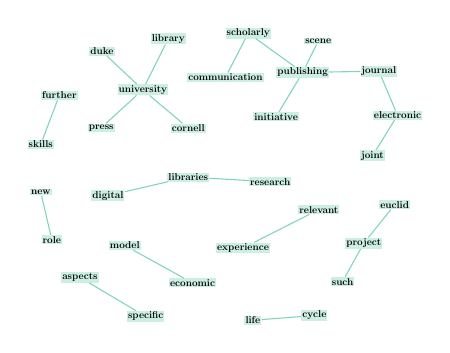
\begin{tikzpicture}[thin,
                              auto,
                              scale=.25,
                              align=center,
                              node distance=2cm,
                              every node/.style={font=\small, transform shape},
                              main node/.style={text centered,
                                                thick,
                                                fill=JungleGreen!20,
                                                inner sep=1.5pt,
                                                font=\Large\bfseries}]
            % connected component
            \node[main node] (university) {university};
            \node[main node] (duke) [above left=of university.north] {duke};
            \node[main node] (library) [above=of university.north east] {library};
            \node[main node] (press) [below left=of university.south] {press};
            \node[main node] (cornell) [below right=of university.south] {cornell};

            \path[JungleGreen!50] (university) edge (library);
            \path[JungleGreen!50] (university) edge (duke);
            \path[JungleGreen!50] (university) edge (press);
            \path[JungleGreen!50] (university) edge (cornell);

            % connected component
            \node[main node] (further) [left=of university.south west] {further};
            \node[main node] (skills) [below=of further.south west] {skills};

            \path[JungleGreen!50] (skills) edge (further);

            % connected component
            \node[main node] (scholarly) [right=of library.north east] {scholarly};
            \node[main node] (communication) [below=of scholarly.west] {communication};
            \node[main node] (publishing) [below right=of scholarly.south] {publishing};
            \node[main node] (scene) [above right=of publishing.west] {scene};
            \node[main node] (initiative) [below=of publishing.west] {initiative};
            \node[main node] (journal) [below right=of scene.north east] {journal};
            \node[main node] (electronic) [below=of journal.east] {electronic};
            \node[main node] (joint) [below=of electronic.north west] {joint};

            \path[JungleGreen!50] (communication) edge (scholarly);
            \path[JungleGreen!50] (publishing) edge (scholarly);
            \path[JungleGreen!50] (publishing) edge (scene);
            \path[JungleGreen!50] (publishing) edge (journal);
            \path[JungleGreen!50] (publishing) edge (initiative);
            \path[JungleGreen!50] (journal) edge (electronic);
            \path[JungleGreen!50] (joint) edge (electronic);

            % connected component
            \node[main node] (new) [below=of skills.south] {new};
            \node[main node] (role) [below=of new.south east] {role};

            \path[JungleGreen!50] (new) edge (role);

            % connected component
            \node[main node] (digital) [right=of new.south east] {digital};
            \node[main node] (libraries) [below =of cornell.south] {libraries};
            \node[main node] (research) [right =of libraries.south east] {research};

            \path[JungleGreen!50] (digital) edge (libraries);
            \path[JungleGreen!50] (libraries) edge (research);

            % connected component
            \node[main node] (relevant) [below right=of research.north] {relevant};
            \node[main node] (experience) [below left=of relevant.south west] {experience};

            \path[JungleGreen!50] (relevant) edge (experience);

            % connected component
            \node[main node] (model) [below=of digital.south east] {model};
            \node[main node] (economic) [below right=of model.south east] {economic};

            \path[JungleGreen!50] (model) edge (economic);

            % connected component
            \node[main node] (specific) [below left=of economic.center] {specific};
            \node[main node] (aspects) [above left=of specific.north west] {aspects};

            \path[JungleGreen!50] (specific) edge (aspects);

            % connected component
            \node[main node] (life) [below right=of economic.south east] {life};
            \node[main node] (cycle) [right=of life.north east] {cycle};

            \path[JungleGreen!50] (life) edge (cycle);

            % connected component
            \node[main node] (euclid) [right=of relevant.north east] {euclid};
            \node[main node] (project) [below left=of euclid.south east] {project};
            \node[main node] (such) [below left=of project.south east] {such};

            \path[JungleGreen!50] (euclid) edge (project);
            \path[JungleGreen!50] (project) edge (such);
          \end{tikzpicture}
        }
      \end{column}
      \begin{column}{.4\textwidth}
        \alt<5->{
          \resizebox{\linewidth}{!}{
            \begin{tabular}{l}
              Extracted Keyphrases\\
              \midrule
              electronic journal publishing\\
              \cellcolor{pink}scholarly publishing\\
              libraries\\
              university\\
              project\\
              economic\\
              relevant\\
              role
            \end{tabular}
          }
        }{
          \uncover<4>{
            \resizebox{\linewidth}{!}{
              \begin{tabular}{l}
                Extracted Keyphrases\\
                \midrule
                electronic journal publishing\\
                scholarly publishing\\
                libraries\\
                university\\
                project\\
                economic\\
                relevant\\
                role
              \end{tabular}
            }
          }
        }
      \end{column}
    \end{columns}

    \begin{block}<6->{Drawbacks}
      \begin{itemize}
        \item{Word nodes}
        \item{Co-occurence window}
        \item{Several nodes for one topic}
      \end{itemize}
    \end{block}
  \end{frame}


  %\section{This Work}
  \begin{frame}[t]{This Work}
    \begin{block}{Limitations of previous work}
      \begin{itemize}
        \item{Word nodes\tikz[overlay, remember picture]\node[coordinate, xshift=.5em, yshift=.25em] (b1) {};}
        \item{\tikz[overlay, remember picture]\node[coordinate, xshift=-.5em, yshift=.25em] (b2) {};Co-occurence window}
        \item{Several nodes for one topic\tikz[overlay, remember picture]\node[coordinate, xshift=0.5em, yshift=.25em] (b3) {};}
      \end{itemize}
    \end{block}

    \vfill

    \uncover<2->{
      \begin{block}{Proposal}
        \begin{enumerate}
          \item{Topic nodes\tikz[overlay, remember picture]\node[coordinate, xshift=.5em, yshift=.25em] (e1) {};}
          \item<3->{\tikz[overlay, remember picture]\node[coordinate, xshift=-.5em, yshift=.25em] (e2) {};Complete graph construction}
          \item<4->{Selection of one keyphrase representing each topic}
        \end{enumerate}
      \end{block}
    }

    \visible<2->{
      \begin{tikzpicture}[overlay, remember picture]
        \draw[->, thick] (b1) .. controls ([xshift=7cm] b1) and ([xshift=5cm] e1) .. (e1);
        \draw[->, thick] (b3) .. controls ([xshift=2cm] b3) and ([xshift=3cm] e1) .. (e1);
      \end{tikzpicture}
    }
    \visible<3->{
      \begin{tikzpicture}[overlay, remember picture]
        \draw[->, thick] ([xshift=-.5cm] b2) .. controls ([xshift=-1.25cm] b2) and ([xshift=-1.25cm] e2) .. ([xshift=-.5cm] e2);
      \end{tikzpicture}
    }
  \end{frame}


  \begin{frame}{Plan}
    \tableofcontents
  \end{frame}
  \AtBeginSection[]{
    \begin{frame}{Plan}
      \tableofcontents[currentsection]
    \end{frame}
  }
  \section{Extraction de termes-clés avec TopicRank}
\label{sec:extraction_de_termes_cles_avec_topicrank}
  \begin{itemize}
    \item{principe général}
    \item{identification des sujets}
    \item{ordonancement des sujets}
    \begin{itemize}
      \item{construction du graphe de sujets}
      \item{ordonnancement dans le graphe de sujets}
    \end{itemize}
    \item{selection des termes-clés}
  \end{itemize}


  \section{Experimental Settings}
\label{sec:experimental_settings}
  \subsection{Dataset}
  \label{subsec:dataset}
    In this work, we use the SemEval corpus. Built for the task 5 of
    SemEval-2010~\cite{kim2010semeval}, Sem\-Eval contains 244 English
    scientific papers collected from the ACM Digital Libraries. We use
    Sem\-Eval's training set (144 documents) and test set (100 documents) with
    their sets of combined author- and reader-assigned keyphrases.

  \subsection{Baselines}
  \label{subsec:baselines}
    In order to show that our method benefits from all aspects of its
    configuration, we design a set of baselines that slightly diverge from our
    method (deried baselines). First, To\-picRank plus the SVM classifier
    trained on either topically independent and dependent features
    (TopicRank+SVM), while the SVM classifier is trained on all features for our
    method (TopicRank+SVM$_{all}$). Second the SVM classifier, trained on either
    topically independent, dependent or all features, is applied to the unranked
    clusters (Clustering+SVM). Finally, the SVM classifier, trained on topically
    independent features, is applied candidate keyphrases (SVM).

    For comparison purpose, we also report results of a Naive Bayes classifier
    trained with the first position and the TF-IDF
    features~\cite[KEA]{witten1999kea}, TF-IDF and TopicRank.

  \subsection{Preprocessing}
  \label{subsec:preprocessing}
%    For each document, we apply the following preprocessing steps: sentence
%    segmentation, word tokenization and Part-of-Speech tagging. For sentence
%    segmentation, we use the PunktSentenceTokenizer provided by the Python
%    Natural Language ToolKit~\cite[NLTK]{bird2009nltk}. For word tokenization,
%    we use the NLTK TreebankWordTokenizer for English and the Bonsai word
%    tokenizer\footnote{The Bonsai word tokenizer is a tool provided with the
%    Bonsai PCFG-LA parser:
%    \url{http://alpage.inria.fr/statgram/frdep/fr_stat_dep_parsing.html}.} for
%    French. As for Part-of-Speech tagging, we use the Stanford POS
%    tagger~\cite{toutanova2003stanfordpostagger} for English and
%    MElt~\cite{denis2009melt} for French.
    %%%%%%%%%%%%%%%%%%%%%%%%%%%%%%%%%%%%%%%%%%%%%%%%%%%%%%%%%%%%%%%%%%%%%%%%%%%%
    For our method, as well as all baselines, we use Topic\-Rank's outputs.
    Therefore, our results can directly be compared to results
    in~\cite{bougouin2013topicrank}.

  \subsection{Evaluation Measures}
  \label{subsec:evaluation_measures}
    We evaluate the performances of our method and the baselines in terms of
    precision (P), recall (R) and f-score (f1-measure, F) when at most 10
    keyphrases are extracted. In order to reduce mismatches due to flexions such
    as plural, we also stem candidate and reference keyphrases during the
    evaluation.

\section{Results}
\label{sec:results}
  Figure~\ref{fig:baseline_comparison} presents the performance of our method,
  compared to six baselines derived from it. On the first hand, we observe that
  using clusters and their importance score benefits to the keyphrase
  extraction. Most importantly, adding topically dependent features to the
  common features improves the performance. However, the performance achieved
  with the Clustering+SVM method shows that topically dependent features
  performs poorly when Topic\-Rank's importance score is not used. Additionally,
  the SVM performance tends to show that using clusters without taking their
  importance into account is not relevant. Results support our statement that
  keyphrases should be extracted from important topics.
  \begin{figure}[h]
    \begin{tikzpicture}%[scale=.75]
      \pgfkeys{/pgf/number format/.cd, fixed, fixed zerofill, precision=1}
      \begin{axis}[axis lines=left,
                   symbolic x coords={TopicRank+SVM, Clustering+SVM, SVM},
                   xtick=data,
                   enlarge x limits=0.2,
                   %x=.25\linewidth,
                   xticklabel style={anchor=west, rotate=-22.25},
                   nodes near coords,
                   nodes near coords align={vertical},
                   every node near coord/.append style={font=\scriptsize},
                   ytick={0.0, 5.0, 10.0, 15.0, 20.0, 25.0},
                   y=0.025\linewidth,
                   ymin=0.0,
                   ymax=22.0,
                   ybar=7.5pt,
                   ylabel=F,
                   ylabel style={at={(ticklabel* cs:1)},
                                 anchor=south,
                                 rotate=270},
                   legend style={at={(1.0, 1.0)},
                                 anchor=north east}]
        \addplot[Cerulean,
                 pattern=north east lines,
                 pattern color=Cerulean] coordinates{
          (SVM, 12.2)
          (Clustering+SVM, 10.8)
          (TopicRank+SVM, 17.6)
        };
        \addplot[YellowGreen,
                 pattern=north west lines,
                 pattern color=YellowGreen] coordinates{
          (SVM, 0.0)
          (Clustering+SVM, 0.2)
          (TopicRank+SVM, 7.5)
        };
        \addplot[RedOrange,
                 pattern=horizontal lines,
                 pattern color=RedOrange] coordinates{
          (SVM, 0.0)
          (Clustering+SVM, 9.7)
          (TopicRank+SVM, 19.6)
        };
        \legend{Independent features, Dependent features, All features}
      \end{axis}
    \end{tikzpicture}
    \caption{Performance of TopicRank+SVM$_{all}$ compared to derived baselines
             \label{fig:baseline_comparison}}
  \end{figure}

  Also, Table~\ref{tab:state_of_the_art_comparison} presents a comparison of
  TopicRank+SVM$_{all}$ with TopicRank, TopicRank's best possible performance
  (TopicRank$_{max}$) and common baselines of previous work. Results show that
  our method significantly improves TopicRank and significantly outperform
  TF-IDF and KEA, a robust supervised methods. However, the performance of
  TopicRank+SVM$_{all}$ is still very low compared to the best possible
  performance that could be achieved with TopicRank. The naivety of the
  clustering method TopicRank applies may introduce noise that dampens the
  performance. Future improvement should focus on a more efficient clustering of
  the candidates belonging to the same topic.
  \begin{table}[h]
    \centering
    \begin{tabular}{|r|rrr|}
      \hline
      Method & \multicolumn{1}{c}{P} & \multicolumn{1}{c}{R} & \multicolumn{1}{c|}{F}\\
      \hline
      KEA                   & 18.8\textcolor{white}{$^\dagger$} & 13.3\textcolor{white}{$^\dagger$} & 15.4\textcolor{white}{$^\dagger$}\\
      TF-IDF                & 13.2\textcolor{white}{$^\dagger$} & 8.9\textcolor{white}{$^\dagger$} & 10.5\textcolor{white}{$^\dagger$}\\
      TopicRank             & 14.9\textcolor{white}{$^\dagger$} & 10.3\textcolor{white}{$^\dagger$} & 12.1\textcolor{white}{$^\dagger$}\\
      TopicRank+SVM$_{all}$ & 24.2$^\dagger$ & 16.7$^\dagger$ & 19.6$^\dagger$\\
      \hline
      TopicRank$_{max}$     & 37.6\textcolor{white}{$^\dagger$} & 25.8\textcolor{white}{$^\dagger$} & 30.3\textcolor{white}{$^\dagger$}\\
      \hline
    \end{tabular}
    \caption{Performance of TopicRank+SVM$_{all}$ compared to previous work.
      $\dagger$ indicates improvement over KEA, TF-IDF and TopicRank at 0.001
      level using Student's t-test.
             \label{tab:state_of_the_art_comparison}}
  \end{table}

%\section{Error Analysis}
%\label{sec:error_analysis}


  \section{Conclusion and Future Work}
  \begin{frame}{Conclusion and Future Work}

    What is done?
    \begin{itemize}
      \item{Proposed TopicRank}
      \item{Topic ranking instead of word ranking}
      \item{Complete graph}
      \item{Experiments conducted of four standard datasets}
      \item{Good results}
      \item{Promising upper bound results}
    \end{itemize}

    \vfill

    \uncover<2->{
      Still to do?
      \begin{itemize}
        \item{Experiment various topic identifications}
        \item{Provide a keyphrase selection strategy getting closer to the upper bound}
      \end{itemize}
    }
  \end{frame}


  \begin{frame}
    \vfill
    \begin{beamercolorbox}[center,shadow=true,rounded=true]{frametitle} 
      \Huge{\textbf{Thank you}}
    \end{beamercolorbox} 
    \vfill
  \end{frame}
  %\section{Backups}
  \begin{frame}[label=candidate_clustering_backup]{Backups}
    \framesubtitle{\hyperlink{topicrank}{Candidate Clustering}}

    The hierarchical clustering is an iterative algorithm:
    \begin{itemize}
      \item{Initial state: candidates keyphrases are clusters}
      \item{Clusters with the highest similarity are merged together}
      \item{Clusters similarity is the average similarity between their
            candidates $c_i$:}
      \begin{align}
        \text{similarity}(c_1, c_2) = \frac{||\text{stem}(c_1) \cap \text{stem}(c_2)||}{||\text{stem}(c_1)  \cup \text{stem}(c_2)||} \notag
      \end{align}
      \item{A similarity threshold is set to 0.25}
    \end{itemize}
  \end{frame}

  \begin{frame}[label=graph_construction_backup]{Backups}
    \framesubtitle{\hyperlink{topicrank}{Graph Construction}}

    \begin{itemize}
      \item{Nodes are topics}
      \item{Every nodes are connected to each other}
      \item{Connections between topics are weighted by the semantic strength
            between them}
      \item{Topics appearing close to each other have a high semantic strength:}
    \end{itemize}

    \begin{small}
      \begin{align}
        \text{weight}(t_i, t_j) &= \mathlarger{\sum}_{c_i \in t_i}\ \mathlarger{\sum}_{c_j \in t_j} \text{dist}(c_i, c_j) \notag\\
        \text{dist}(c_i, c_j) &= \mathlarger{\sum}_{p_i \in \text{pos}(c_i)}\ \mathlarger{\sum}_{p_j \in \text{pos}(c_j)} \frac{1}{|p_i - p_j|} \notag
      \end{align}
    \end{small}
  \end{frame}

  \begin{frame}[label=topic_ranking_backup]{Backups}
    \framesubtitle{\hyperlink{topicrank}{Topic Ranking}}

    \begin{block}{PageRank's ``voting'' concept}
      High-scoring topics contribute more to the score of their connected
      topics.
    \end{block}

    \begin{align}
      \text{Score}(t_i) = (1 - \lambda) + \lambda \times \sum_{t_j \neq t_i} \frac{\text{weight}(t_i, t_j) \times \text{Score}(t_j)}{\mathlarger{\sum}_{t_k \neq t_j} \text{weight}(t_j, t_k)} \notag
    \end{align}
  \end{frame}

  \begin{frame}[label=main_results_backup]{Backups}
    \framesubtitle{\hyperlink{main_results}{Main Results}}

    \resizebox{\linewidth}{!}{
      \begin{tabular}{rcccccccccccc}
        \toprule
        \multirow{2}{*}[-2pt]{\textbf{Methods}} & \multicolumn{3}{c}{\textbf{Inspec}} & \multicolumn{3}{c}{\textbf{SemEval}} & \multicolumn{3}{c}{\textbf{WikiNews}} & \multicolumn{3}{c}{\textbf{DEFT}}\\
        \cmidrule(lr){2-4}\cmidrule(lr){5-7}\cmidrule(lr){8-10}\cmidrule(l){11-13}
        & P & R & F & P & R & F & P & R & F & P & R & F\\
        \midrule
        TF-IDF & 32.7 & 38.6 & 33.4 & 13.2 & $~~$8.9 & 10.5 & 33.9 & 35.9 & 34.3 & 10.3 & 19.1 & 13.2\\
        TextRank & 14.2 & 12.5 & 12.7 & $~~$7.9 & $~~$4.5 & $~~$5.6 & $~~$9.3 & $~~$8.3 & $~~$8.6 & $~~$4.9 & $~~$7.1 & $~~$5.7\\
        SingleRank & \cellcolor{pink}{34.8} & \cellcolor{pink}{40.4} & \cellcolor{pink}{35.2} & $~~$4.6 & $~~$3.2 & $~~$3.7 & 19.4 & 20.7 & 19.7 & $~~$4.5 & $~~$9.0 & $~~$5.9\\
        TopicRank & 27.6 & 31.5 & 27.9  & \cellcolor{pink}{14.9} & \cellcolor{pink}{10.3} & \cellcolor{pink}{12.1} & \cellcolor{pink}{35.0} & \cellcolor{pink}{37.5} & \cellcolor{pink}{35.6} & \cellcolor{pink}{11.7} & \cellcolor{pink}{21.7} & \cellcolor{pink}{15.1}\\
        \bottomrule
      \end{tabular}
    }
  \end{frame}

  \begin{frame}[label=contributions_evaluation_backup]{Backups}
    \framesubtitle{\hyperlink{contributions_evaluation}{Contributions Evaluation}}

    \resizebox{\linewidth}{!}{
      \begin{tabular}{rcccccccccccc}
        \toprule
        \multirow{2}{*}[-2pt]{\textbf{Methods}} & \multicolumn{3}{c}{\textbf{Inspec}} & \multicolumn{3}{c}{\textbf{SemEval}} & \multicolumn{3}{c}{\textbf{WikiNews}} & \multicolumn{3}{c}{\textbf{DEFT}}\\
        \cmidrule(lr){2-4}\cmidrule(lr){5-7}\cmidrule(lr){8-10}\cmidrule(l){11-13}
        & P & R & F & P & R & F & P & R & F & P & R & F\\
        \midrule
        SingleRank & 34.8 & 40.4 & 35.2 & $~~$4.6 & $~~$3.2 & $~~$3.7 & 19.4 & 20.7 & 19.7 & $~~$4.5 & $~~$9.0 & $~~$5.9\\
        +phrases & 21.5 & 25.9 & 22.1 & $~~$9.6 & $~~$7.0 & $~~$8.0 & 28.6 & 30.1 & 28.9 & 10.5 & 19.7 & 13.5\\
        +topics & 26.6 & 30.2 & 26.8 & 14.7 & 10.2 & 11.9 & 31.0 & 32.8 & 31.4 & 11.5 & 21.4 & 14.8\\
      +complete & \cellcolor{pink}{34.9} & \cellcolor{pink}{41.0} & \cellcolor{pink}{35.5} & $~~$5.5 & $~~$3.8 & $~~$4.4 & 20.0 & 21.4 & 20.3${~}$ & $~~$4.4 & $~~$9.0 & $~~$5.8\\
      TopicRank & 27.6 & 31.5 & 27.9  & \cellcolor{pink}{14.9} & \cellcolor{pink}{10.3} & \cellcolor{pink}{12.1} & \cellcolor{pink}{35.0} & \cellcolor{pink}{37.5} & \cellcolor{pink}{35.6} & \cellcolor{pink}{11.7} & \cellcolor{pink}{21.7} & \cellcolor{pink}{15.1}\\
        \bottomrule
      \end{tabular}
    }
  \end{frame}

  \begin{frame}[label=keyphrase_selection_evaluation_backup]{Backups}
    \framesubtitle{\hyperlink{keyphrase_selection_evaluation}{Keyphrase Selection Evaluation}}

    \resizebox{\linewidth}{!}{
      \begin{tabular}{rcccccccccccc}
        \toprule
        \multirow{2}{*}[-2pt]{\textbf{Keyphrase selection}} & \multicolumn{3}{c}{\textbf{Inspec}} & \multicolumn{3}{c}{\textbf{SemEval}} & \multicolumn{3}{c}{\textbf{WikiNews}} & \multicolumn{3}{c}{\textbf{DEFT}}\\
        \cmidrule(lr){2-4}\cmidrule(lr){5-7}\cmidrule(lr){8-10}\cmidrule(l){11-13}
        & P & R & F & P & R & F & P & R & F & P & R & F\\
        \midrule
        \rowcolor{cyan!33} First position & 27.6 & 31.5 & 27.9  & 14.9 & 10.3 & 12.1 & 35.0 & 37.5 & 35.6 & 11.7 & 21.7 & 15.1\\
        Frequency & 26.7 & 30.2 & 26.8 & $~~$1.7 & $~~$1.2 & $~~$1.4 & 25.7 & 27.6 & 26.2 & $~~$1.9 & $~~$3.8 & $~~$2.5\\
        Centroid & 24.5 & 28.0 & 24.7 & $~~$1.9 & $~~$1.2 & $~~$1.5 & 28.1 & 29.9 & 28.5 & $~~$2.6 & $~~$5.0 & $~~$3.4\\
        \midrule
        \rowcolor{pink} Upper bound & 36.4 & 39.0 & 35.6 & 37.6 & 25.8 & 30.3 & 42.5 & 44.8 & 42.9 & 14.9 & 28.0 & 19.3\\
        \bottomrule
      \end{tabular}
    }
  \end{frame}


  \section*{Références}
    \begin{frame}[allowframebreaks]{References}
      \def\newblock{\hskip .11em plus .33em minus .07em}
      \bibliographystyle{plainnat}
      \bibliography{../../biblio}
    \end{frame}
\end{document}

